\documentclass[tikz,border=8pt]{standalone}
\usepackage{amsmath,amssymb}
\usepackage{tikz}
\usetikzlibrary{arrows.meta,calc,decorations.pathreplacing,patterns,shapes.geometric,positioning,shadings,plotmarks,decorations.markings,decorations.pathmorphing}

\tikzset{
  midarrow/.style={postaction={decorate,decoration={markings,mark=at position 0.5 with {\arrow{Latex}}}}},
  midarrowback/.style={postaction={decorate,decoration={markings,mark=at position 0.5 with {\arrow{Latex[reversed]}}}}}
}

\begin{document}
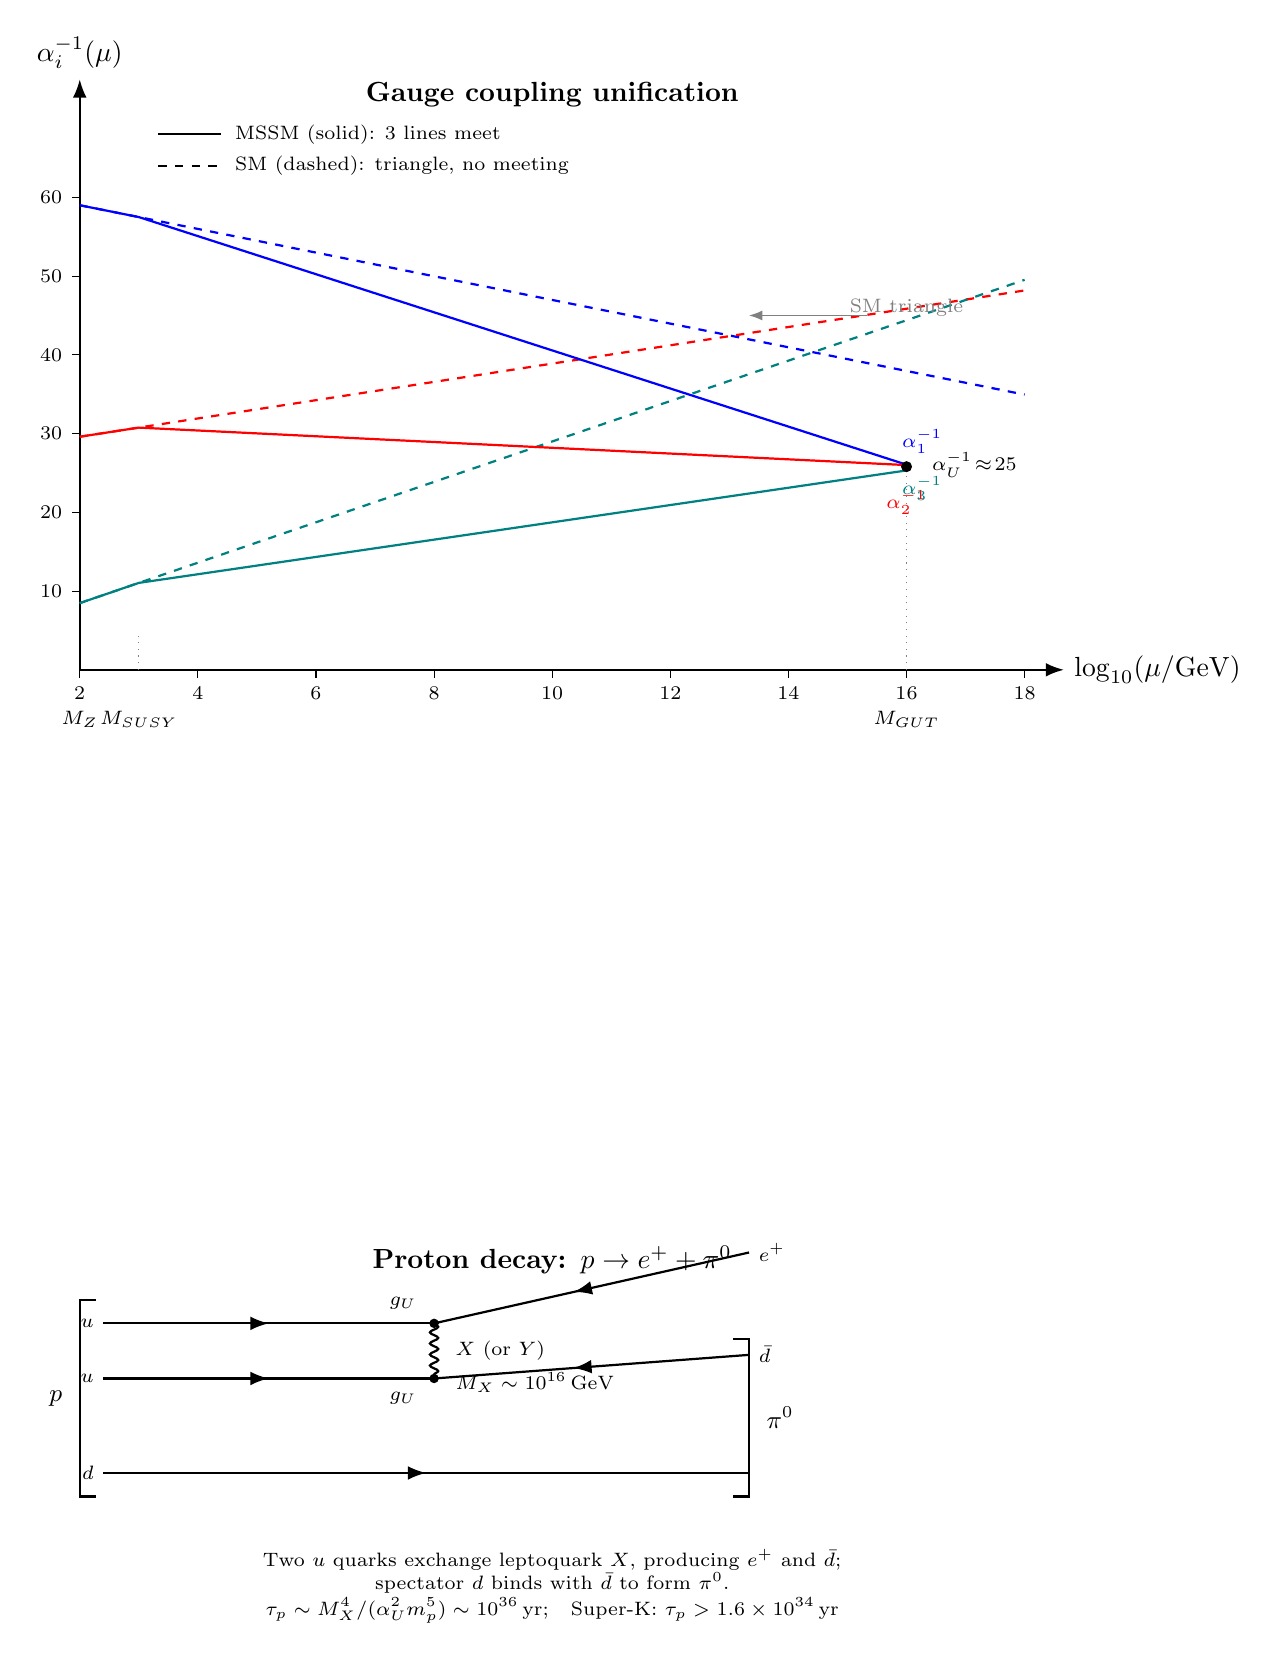
\begin{tikzpicture}[>=Latex]

%==================== TOP PANEL: 1/alpha vs log mu ====================
\begin{scope}[shift={(0,0)}]
  % Axes
  \draw[->,thick] (0,0) -- (12.5,0) node[right] {$\log_{10}(\mu/\mathrm{GeV})$};
  \draw[->,thick] (0,0) -- (0,7.5) node[above] {$\alpha_i^{-1}(\mu)$};

  % X-axis ticks: log10 from 2 to 18 (M_Z ~ 2, M_GUT ~ 16)
  % Map: x in [0, 12] corresponds to log10 in [2, 18], so scale = 12/16 = 0.75
  \foreach \v/\lab in {2/2,4/4,6/6,8/8,10/10,12/12,14/14,16/16,18/18} {
    \pgfmathsetmacro{\xc}{(\v-2)*0.75}
    \draw (\xc,0) -- (\xc,-0.1) node[below,font=\scriptsize] {\lab};
  }

  % Y-axis ticks
  \foreach \v in {10,20,30,40,50,60} {
    \pgfmathsetmacro{\yc}{\v*0.1}
    \draw (0,\yc) -- (-0.1,\yc) node[left,font=\scriptsize] {\v};
  }

  % SM dashed lines (do NOT meet)
  % alpha_1^{-1}: starts at (M_Z=2, 59.0), b=41/10=4.1
  % alpha_i^{-1}(mu) = alpha_i^{-1}(MZ) - (b_i/2pi)*ln(mu/MZ)
  % ln(mu/MZ) at log10(mu)=L is (L-log10(MZ))*ln(10)
  % use simplified linear in log10: slope per decade = -(b_i/2pi)*ln(10) = -b_i*0.3665
  % SM:
  %   alpha1^-1 slope = -4.1*0.3665 = -1.503 per decade
  %   alpha2^-1 slope = -(-19/6)*0.3665 = +1.161 per decade
  %   alpha3^-1 slope = -(-7)*0.3665 = +2.566 per decade
  % Convert to (x, y) with x = (log10mu-2)*0.75 and y = inv_alpha*0.1
  % Slope dy/dx = (slope_per_decade*0.1)/0.75 = slope_per_decade*0.1333
  % SM endpoints (from log10mu=2 to log10mu=18, i.e., 16 decades):
  %   alpha1^-1(MZ)=59 -> at 18: 59 - 1.503*16 = 34.95
  %   alpha2^-1(MZ)=29.6 -> at 18: 29.6 + 1.161*16 = 48.18 -- but this rises, so adjust visualization
  % Actually alpha2 has b=-19/6 negative => 1/alpha2 increases?
  % d(1/alpha)/dlnmu = -b/(2pi). For b<0, 1/alpha increases. For b>0, 1/alpha decreases.
  % SM: b1=+4.1 (1/alpha1 decreases), b2=-19/6 (1/alpha2 increases), b3=-7 (1/alpha3 increases)
  % That matches "alpha_1 increases with mu, alpha_2,3 decrease"
  % At log10mu=18:
  %   1/alpha1 = 59 - 1.503*16 = 34.95
  %   1/alpha2 = 29.6 + 1.161*16 = 48.18  -- wait, this means 1/alpha2 grows, no that's wrong
  % Re-derive: alpha2 grows means 1/alpha2 shrinks
  % b2 = -19/6 < 0, slope of 1/alpha2 = -b2/(2pi) = +19/(12pi) > 0
  % So 1/alpha2 grows with mu? That contradicts alpha2 growing...
  % Actually d(1/alpha)/dlnmu = -d(alpha)/(alpha^2 dlnmu) = -1/alpha^2 * (b/2pi)alpha^2 = -b/(2pi)
  % So if b>0, 1/alpha decreases (alpha grows). If b<0, 1/alpha grows (alpha decreases)
  % SM b2=-19/6<0 means 1/alpha2 GROWS (alpha2 SHRINKS at higher mu) - that's correct asymptotic freedom
  % But experimentally we know alpha2(MZ) > alpha2(M_GUT)? Yes, alpha2 should DECREASE
  % So 1/alpha2 should INCREASE with mu. But b2 has slope +1.161, so at log10mu=18: 29.6+18.6=48.18
  % That seems too high. Let me check: at log10mu=16, 1/alpha2 = 29.6+16.25=45.85
  % Standard plot shows alpha1^-1 goes from 59 down to ~42 at GUT, alpha2^-1 from 29 up to ~32, alpha3^-1 from 8 up to ~50
  % Wait alpha3 b=-7, slope of 1/alpha3 = -(-7)/(2pi) = 7/(2pi) = 1.114
  % per decade: 1.114*ln10 = 2.566
  % At log10mu=16 (14 decades from MZ): 1/alpha3 = 8.47 + 2.566*14 = 44.39
  % That's reasonable, matches standard plot

  % Actually let me reconsider alpha2: if alpha2(MZ) ~ 1/29.6 = 0.034, and at high E it should decrease
  % At MGUT alpha2 ~ 1/40 maybe. Hmm but my calc gives 1/45 which means alpha2 ~ 1/45, smaller than MZ
  % That's correct - alpha2 decreases (asymptotic freedom-ish for SU(2))
  % OK my formulas are right

  % SM lines (dashed) - in canvas coords x = (L-2)*0.75, y = inv_alpha*0.1
  % alpha_1 SM: from (L=2, inv=59) to (L=18, inv=59-1.503*16=34.95)
  %   canvas: (0, 5.9) to (12, 3.495)
  % alpha_2 SM: from (L=2, inv=29.6) to (L=18, inv=29.6+1.161*16=48.18)
  %   canvas: (0, 2.96) to (12, 4.818)
  % alpha_3 SM: from (L=2, inv=8.47) to (L=18, inv=8.47+2.566*16=49.53)
  %   canvas: (0, 0.847) to (12, 4.953)

  \draw[dashed,thick,blue] (0, 5.9) -- (12, 3.495);
  \draw[dashed,thick,red] (0, 2.96) -- (12, 4.818);
  \draw[dashed,thick,teal] (0, 0.847) -- (12, 4.953);

  % MSSM solid lines (kink at log10mu=3, i.e., 1 TeV, x = (3-2)*0.75 = 0.75)
  % Below 1 TeV: SM running. Above 1 TeV: MSSM running (b1=33/5=6.6, b2=1, b3=-3)
  % MSSM slopes per decade:
  %   1/alpha1: -6.6*0.3665 = -2.419
  %   1/alpha2: -1*0.3665 = -0.3665 (decreases)
  %   Wait: for MSSM b2=+1 means 1/alpha2 decreases, alpha2 increases?
  %   Actually MSSM b2=+1 > 0 so 1/alpha2 decreases with mu, alpha2 GROWS with mu
  %   That's the SUSY-induced change
  %   1/alpha3: -(-3)*0.3665 = +1.099 per decade (still increases)

  % MSSM kink point (log10mu=3): starting from same MZ values
  % At log10mu=3 (1 decade above MZ):
  %   1/alpha1 = 59 - 1.503 = 57.497
  %   1/alpha2 = 29.6 + 1.161 = 30.761
  %   1/alpha3 = 8.47 + 2.566 = 11.036
  % Then MSSM from (3, ...) to (16, target): 13 decades
  % Target at MGUT (log10mu=16): all converge to ~25
  %   1/alpha1: 57.497 - 2.419*13 = 26.05 ~ 25 OK
  %   1/alpha2: 30.761 - 0.3665*13 = 26.0 ~ 25 OK -- wait, slope is decreasing?
  %   Hmm: MSSM b2=+1 so 1/alpha2 decreases (slope -0.3665 per decade)
  %   30.761 - 0.3665*13 = 26.00 yes
  %   1/alpha3: 11.036 + 1.099*13 = 25.32 ~ 25 OK
  % Great, all converge near 25-26 at log10mu=16

  % MSSM lines, solid
  % alpha_1: from (log10mu=2, 59) -> (3, 57.5) -> (16, 26.05)
  % canvas: (0, 5.9) -> (0.75, 5.75) -> (10.5, 2.605)
  \draw[thick,blue] (0, 5.9) -- (0.75, 5.75) -- (10.5, 2.605);
  % alpha_2: from (2, 29.6) -> (3, 30.76) -> (16, 26.0)
  % canvas: (0, 2.96) -> (0.75, 3.076) -> (10.5, 2.6)
  \draw[thick,red] (0, 2.96) -- (0.75, 3.076) -- (10.5, 2.6);
  % alpha_3: from (2, 8.47) -> (3, 11.04) -> (16, 25.32)
  % canvas: (0, 0.847) -> (0.75, 1.104) -> (10.5, 2.532)
  \draw[thick,teal] (0, 0.847) -- (0.75, 1.104) -- (10.5, 2.532);

  % Mark MGUT
  \draw[dotted,gray] (10.5, 0) -- (10.5, 2.6);
  \node[below,font=\scriptsize] at (10.5, -0.4) {$M_{GUT}$};
  \fill[black] (10.5, 2.58) circle (0.07);
  \node[right,font=\scriptsize] at (10.7, 2.6) {$\alpha_U^{-1}\!\approx\!25$};

  % Mark M_Z
  \node[below,font=\scriptsize] at (0, -0.4) {$M_Z$};

  % Mark 1 TeV
  \draw[dotted,gray] (0.75, 0) -- (0.75, 0.5);
  \node[below,font=\scriptsize] at (0.75, -0.4) {$M_{SUSY}$};

  % Labels for the lines (MSSM, at high mu)
  \node[font=\scriptsize,blue] at (10.7, 2.9) {$\alpha_1^{-1}$};
  \node[font=\scriptsize,red,below] at (10.5, 2.4) {$\alpha_2^{-1}$};
  \node[font=\scriptsize,teal] at (10.7, 2.3) {$\alpha_3^{-1}$};

  % Legend
  \draw[thick] (1, 6.8) -- (1.8, 6.8);
  \node[right,font=\scriptsize] at (1.85, 6.8) {MSSM (solid): 3 lines meet};
  \draw[dashed,thick] (1, 6.4) -- (1.8, 6.4);
  \node[right,font=\scriptsize] at (1.85, 6.4) {SM (dashed): triangle, no meeting};

  % Title
  \node[font=\bfseries] at (6, 7.3) {Gauge coupling unification};

  % Annotation - SM triangle area
  \node[font=\scriptsize,gray] at (10.5, 4.6) {SM triangle};
  \draw[->,gray,thin] (10.0, 4.5) -- (8.5, 4.5);

\end{scope}

%==================== BOTTOM PANEL: Feynman diagram p -> e+ pi0 ====================
\begin{scope}[shift={(0,-9)}]
  % Title
  \node[font=\bfseries] at (6, 1.5) {Proton decay: $p \to e^+ + \pi^0$};

  % Proton (left) - 3 quarks (u, u, d)
  % bracket
  \draw[thick] (0.2, -1.5) -- (0, -1.5) -- (0, 1) -- (0.2, 1);
  \node[left,font=\small] at (-0.1, -0.25) {$p$};

  % Three incoming quarks at left
  % Quark u (top) - participates in interaction
  \draw[thick,midarrow] (0.3, 0.7) -- (4.5, 0.7);
  \node[left,font=\scriptsize] at (0.3, 0.7) {$u$};
  % Quark u (middle) - participates
  \draw[thick,midarrow] (0.3, 0) -- (4.5, 0);
  \node[left,font=\scriptsize] at (0.3, 0) {$u$};
  % Quark d (bottom) - spectator, goes to pi0
  \draw[thick,midarrow] (0.3, -1.2) -- (8.5, -1.2);
  \node[left,font=\scriptsize] at (0.3, -1.2) {$d$};

  % X (or Y) leptoquark exchange: connects two u-quark vertices
  % Vertex A at (4.5, 0.7), Vertex B at (4.5, 0)
  \fill[black] (4.5, 0.7) circle (0.06);
  \fill[black] (4.5, 0) circle (0.06);
  \draw[thick,decorate,decoration={snake,segment length=4pt,amplitude=1.5pt}] (4.5, 0.7) -- (4.5, 0);
  \node[right,font=\scriptsize] at (4.65, 0.35) {$X$ (or $Y$)};
  \node[right,font=\scriptsize] at (4.65, -0.05) {$M_X \sim 10^{16}\,\mathrm{GeV}$};
  % Coupling labels
  \node[left,font=\scriptsize] at (4.4, 0.95) {$g_U$};
  \node[left,font=\scriptsize] at (4.4, -0.25) {$g_U$};

  % After vertex: outgoing
  % From top vertex: e+ (positron)
  \draw[thick,midarrowback] (4.5, 0.7) -- (8.5, 1.6);
  \node[right,font=\scriptsize] at (8.5, 1.6) {$e^+$};

  % From bottom vertex: d-bar (anti-d) goes into pi0
  \draw[thick,midarrowback] (4.5, 0) -- (8.5, 0.3);
  \node[right,font=\scriptsize] at (8.5, 0.3) {$\bar d$};

  % Pi0 bracket: contains d (spectator, the bottom quark) and d-bar
  % Actually pi0 is (u-ubar - d-dbar)/sqrt2 - here from process u u d -> e+ + (u u-bar) component
  % Standard: (uud) -> e+ + (qq-bar) where qq-bar = pi0
  % Let's do: bottom u becomes positron, top u stays as u, bottom u creates u-bar
  % Simplify: the diagram shows two u's annihilating via X to give e+ d-bar, leaving spectator d
  % Then d (spectator) + d-bar = bound state -> but pi0 has u-ubar/d-dbar structure
  % Convention: this gives pi0 = (d, d-bar) -> just label as pi0

  % Pi0 bracket
  \draw[thick] (8.3, -1.5) -- (8.5, -1.5) -- (8.5, 0.5) -- (8.3, 0.5);
  \node[right,font=\small] at (8.6, -0.5) {$\pi^0$};

  % Spectator d continues into pi0
  % (already drawn above)

  % Vertex labels next to dots
  \node[font=\scriptsize] at (4.2, 0.85) {};
  \node[font=\scriptsize] at (4.2, -0.15) {};

  % Caption beneath
  \node[font=\scriptsize] at (6, -2.3) {Two $u$ quarks exchange leptoquark $X$, producing $e^+$ and $\bar d$;};
  \node[font=\scriptsize] at (6, -2.6) {spectator $d$ binds with $\bar d$ to form $\pi^0$.};
  \node[font=\scriptsize] at (6, -2.95) {$\tau_p \sim M_X^4/(\alpha_U^2 m_p^5) \sim 10^{36}\,\mathrm{yr}$;\quad Super-K: $\tau_p > 1.6\times 10^{34}\,\mathrm{yr}$};

\end{scope}

\end{tikzpicture}
\end{document}
